\documentclass[a4paper,12pt,leqno]{article}
\usepackage[utf8]{inputenc}
\usepackage[T1]{fontenc}
\usepackage[polish]{babel}
\usepackage{a4wide}
\usepackage{graphicx}
\usepackage{subfig}
\usepackage{wrapfig}

\title{\textbf{Algorytmy ewolucyjne}\\
       {\Large Raport z zadania pierwszego}\\[-1ex]}
\author{Karol Konaszyński i Wiktor Janas}
\date{Wrocław, dnia \today\ r.}

\begin{document}
\maketitle
a b c d a b c d a b c d a b c d a b c d a b c d a b c d a b c d a b c d a b c d a b c d a b c d a b c d a b c d a b c d a b c d a b c d 
a b c d a b c d a b c d a b c d a b c d a b c d a b c d a b c d a b c d a b c d a b c d a b c d a b c d a b c d a b c d a b c d a b c d 

\begin{figure}\centering
\footnotesize\include{applemod-vs-fruits}\vspace{-2em}
\normalsize\caption{Dopasowanie owoców (\texttt{fruits}) do obróconego jabłka (\texttt{applemod}); uśrednione wyniki z dziesięciu uruchomień programu.}
\end{figure} 

\begin{figure}\centering
\footnotesize\include{square-vs-romb-popsize}\vspace{-2em}
\normalsize\caption{Wpływ rozmiaru populacji na ewolucję (dopasowanie \texttt{square} do \texttt{romb}); uśrednione wyniki z dziesięciu uruchomień programu.}
\end{figure}
\begin{figure}\centering
\footnotesize\include{square-vs-romb-deprop}\vspace{-2em}
\normalsize\caption{Wpływ prawdopodobieństwa krzyżowania na ewolucję (dopasowanie \texttt{square} do \texttt{romb}); uśrednione wyniki dziesięciu uruchomień programu.}
\end{figure}
\begin{figure}\centering
\footnotesize\include{square-vs-romb-surv}\vspace{-2em}
\normalsize\caption{Wpływ współczynnika przetrwania na ewolucję (dopasowanie \texttt{square} do \texttt{romb}); uśrednione wyniki dziesięciu uruchomień programu.}
\end{figure}

\begin{figure}\centering
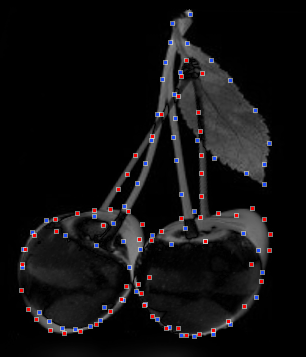
\includegraphics[width=6cm,keepaspectratio=true]{./cherries-match.png}
\caption{Dopasowanie \texttt{cherries} do \texttt{cherries6}}
\end{figure}


\begin{figure}\centering
\subfloat[Jabłko]{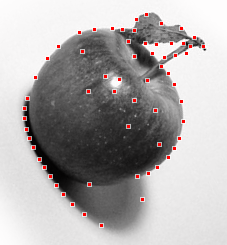
\includegraphics[width=6cm,keepaspectratio=true]{./apple-mod-pois.png}}
\subfloat[Wisienki]{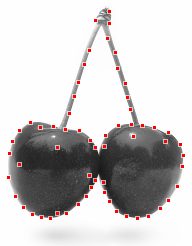
\includegraphics[width=6cm,keepaspectratio=true]{./cherries-pois.png}}\\
\subfloat[Trójliterówka]{
\includegraphics[width=6cm,keepaspectratio=true]{./jeb-pois.png}}
\subfloat[Szum]{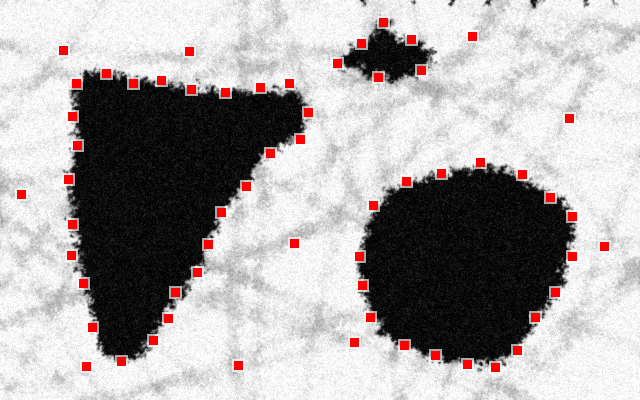
\includegraphics[width=6cm,keepaspectratio=true]{./noisy-pois.png}}
\caption{Obrazy testowe}
\end{figure}

\end{document}
